\begin{problem}{시간 끌기}
    {표준 입력}{표준 출력}
    {1 초}{512 MB}{}
    
    영희와 철수는 공부하기에 앞서 게임을 하고 있다. 게임은 $ N \times M $ 크기의 게임판에서 진행되는데 몇몇 칸은 X 표시가 있다.
    
    게임은 두 명이 번갈아 가며 진행되고 다음의 규칙을 따른다.
    
    \begin{enumerate}
        \item 아직 선택되지 않은 행 또는 열을 하나 선택하되, 기존에 선택되었던 행과 열과의 교차점에 X가 있어서는 안 된다.
        \item 선택한 후, 상대의 차례가 된다.
        \item 만약 조건을 만족하는 행 또는 열이 없다면 (또는 이미 모든 행 또는 열을 선택했다면) 그 사람은 지고 게임은 끝난다.
    \end{enumerate}
    예를 들어 다음의 게임판을 보자.
    
    \begin{figure}[h]
        \centering
        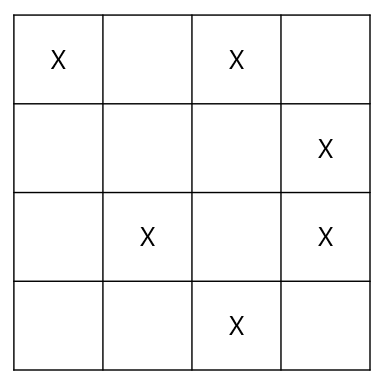
\includegraphics[width=0.25\textwidth]{board.png}
    \end{figure}
    
    지금까지 두 번째 행과 네 번째 행, 두 번째 열을 선택한 상태라고 하자. 그렇다면 첫 번째 행을 선택하거나 네 번째 열을 선택하는 것 외에는 선택된 행, 열들의 교차점에 X가 생기게 된다. 따라서 첫 번째 행이나 첫 번째 열을 선택해야만 하고 그 뒤에는 어떤 행이나 열을 골라도 교차점에 X가 생기므로 총 선택 횟수는 4번이며, 이보다 더 많이 선택할 수 있는 방법은 없다.
    
    철수와 영희는 공부가 매우 하기 싫었기에 누가 이기는지와는 별개로 가장 오래가는 선택을 한다고 가정하자. 이때 철수와 영희는 도합 최대 몇 번의 선택을 할 수 있는지를 출력하시오.
    
    \InputFile
    첫 번째 줄에 게임판의 사이즈인 $ N $과 $ M $, 그리고 X 표시된 칸의 개수 $ K $가 공백으로 구분되어 주어진다. ($ 1 \leq N, M \leq 200 $, $ 1 \leq K \leq NM $)
    
    이후 $ K $개의 줄에 걸쳐 두 자연수 $ x $, $ y $가 공백으로 구분되어 주어진다. ($ 1 \leq x \leq N $, $ 1 \leq y \leq M $) 이는 $ x $행 $ y $열에 있는 칸에 X 표시가 있다는 것을 의미한다.
    
    X 표시가 있는 칸이 중복되어서 입력되는 경우는 없다.
    
    \OutputFile
    첫 번째 줄에 철수와 영희가 합쳐서 총 몇 번의 선택을 하게 되는지 출력한다.
    
    \Examples
    
    \begin{example}
        \exmp{
            4 4 6
            1 1
            1 3
            2 4
            3 2
            3 4
            4 3
        }{%
            4
        }%
    \end{example}
    
\end{problem}

